\section{Results}\label{sec:results}

To draw meaningful conclusions we created several types of visualization of the data. First and foremost we plotted the open events onto a map - either as a point map, e.g Figure \ref{fig:barcelonapoints}, or as a occurrences distribution map for each city district, e.g. Figure \ref{fig:barcelonamap}. Additionally numerous bar charts were created with the number of categories (absolute and per capita) per city, compare Figure \ref{fig:barcelonabar}, and vice versa. 

In this chapter we will shortly discuss several cities and their interesting characteristics. 

\begin{figure}[!htp]
	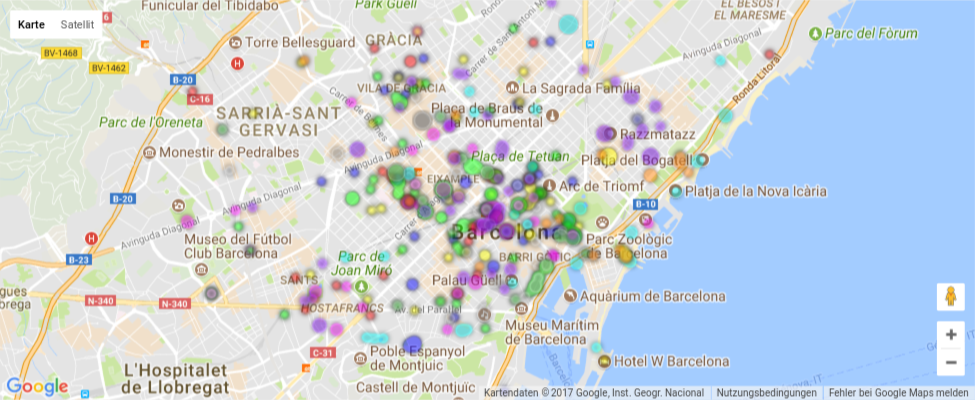
\includegraphics[width=1\linewidth]{images/Barcelona_points.png}
	\caption{Snippet of Barcelona with Open Events}\label{fig:barcelonapoints}	
\end{figure}

\begin{figure}[!htp]
	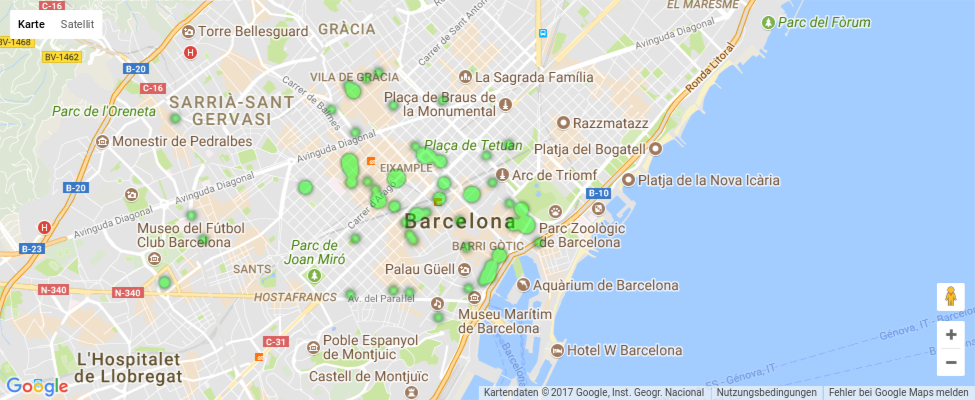
\includegraphics[width=1\linewidth]{images/Barcelona_points_Language.png}
	\caption{Snippet of Barcelona with only Language \& Ethnic Identity Events}\label{fig:barcelonapointslanguage}	
\end{figure}

\begin{figure}[!htp]
	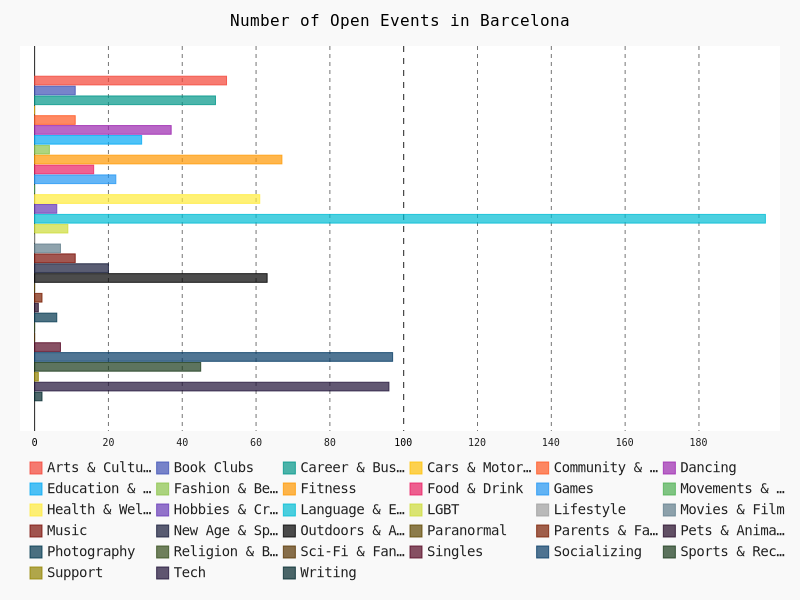
\includegraphics[width=1\linewidth]{../plotting/pngs/categories/Barcelona.png}
	\caption{Activities per Category in Barcelona}\label{fig:barcelonabar}	
\end{figure}

\subsection*{Barcelona}

In Figure \ref{fig:barcelonapoints} one can see an example of Barcelona with open events plotted as points. The different colors represent different Meetup categories. One can see that there are slightly more green points which represent the Meetup category \emph{Language and Ethnic Identity}. A more specific view offers Figure \ref{fig:barcelonapointslanguage} with only the points corresponding to this specific category. Furthermore the already mentioned Chart \ref{fig:barcelonabar} shows that the Language and Ethnic Identity events are indeed the most frequent category which may be an indicator for the diverse and multi-cultural Catalan capital. 

\begin{figure}[!htp]
	% Maximum length
	\subfloat[Activity per District]{\label{fig1:a}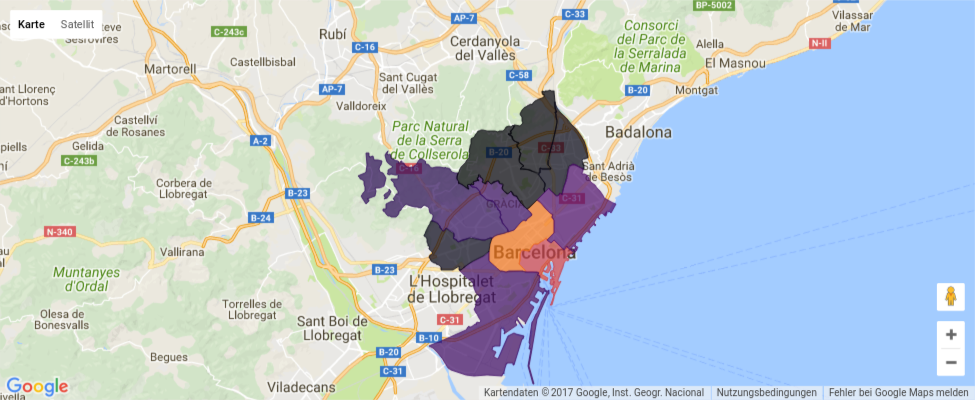
\includegraphics[width=0.49\linewidth]{images/activities_of_districts/Barcelona.png}}\hfill
	\subfloat[Activity per Capita per District]{\label{fig1:b}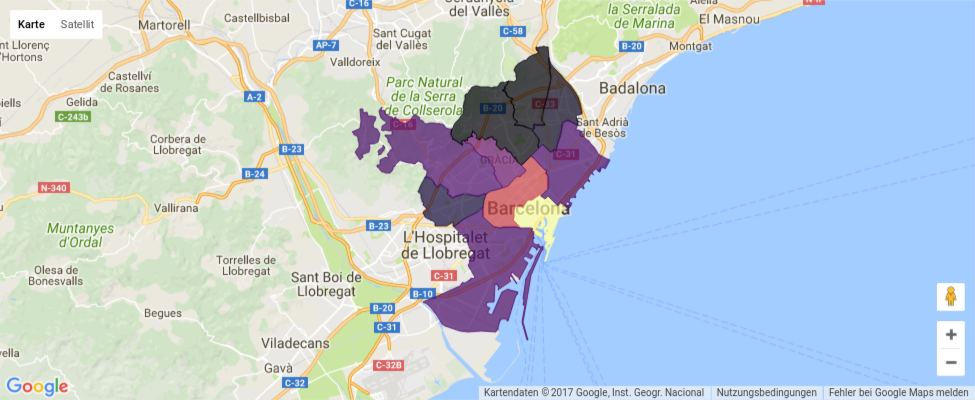
\includegraphics[width=0.49\linewidth]{images/activities_per_capita_of_districts/Barcelona.png}}%
	\caption{Barcelona}\label{fig:barcelonamap}
\end{figure}

The most activities are unsurprisingly in the populous Eixample district but per inhabitant there are more events in Ciutat Vella. Despite having a natural concentration in more centric areas for Barcelona it seems that the activities are a bit more spread out to the whole city. This can be due to Barcelonas small size and its high population density. 
In contrast there are Marid-Centro (Figure \ref{fig:madridmap}), New York-Manhattan (\ref{fig:newyorkmap}) and Hong Kong (\ref{fig:hongkongmap}) where the open events are strongly concentrated in one or a few central districts. 

\subsection*{London}

London seems rather centric with Westminster as the hot-spot district. But especially per capita everything is overshadowed by the small and little populated City of London. Later we will see that London has the highest number of events outside of Europe (in our dataset). 

The most popular categories are Socializing and Tech. 

\begin{figure}[!htp]
	% Maximum length
	\subfloat[Activity per District]{\label{fig1:a}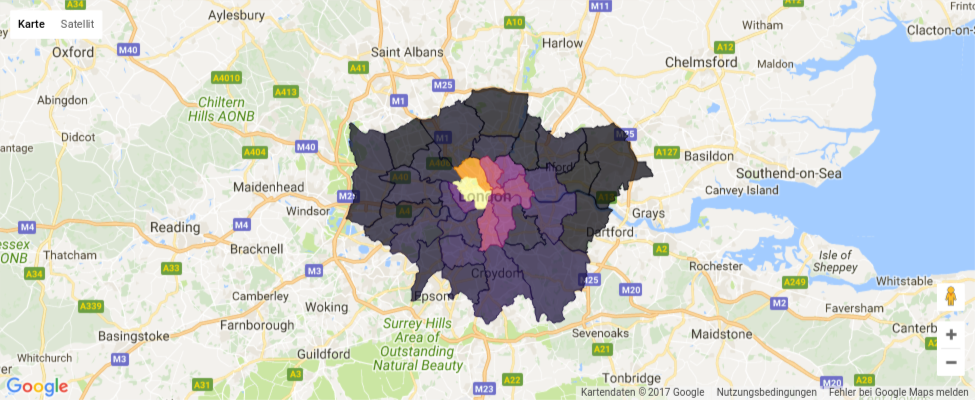
\includegraphics[width=0.49\linewidth]{images/activities_of_districts/London.png}}\hfill
	\subfloat[Activity per Capita per District]{\label{fig1:b}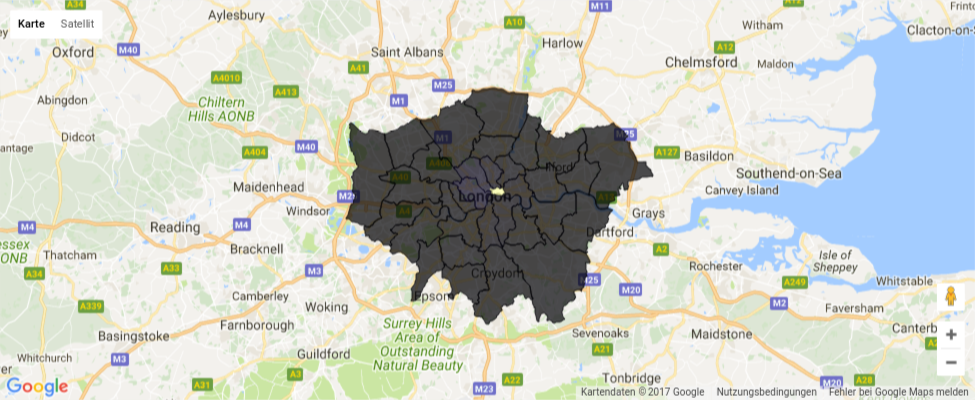
\includegraphics[width=0.49\linewidth]{images/activities_per_capita_of_districts/London.png}}%
	\caption{London}
\end{figure}


\subsection*{Berlin}

Because of the historical division of Berlin it does not have one big city center. One can see (Figure \ref{fig:berlinpoints}) that event concentration is slightly shifted to the east around Prenzlauer Berg (south of Pankow, East of Mitte and Friedrichshain-Kreuzberg. In contrast there is only a smaller focus at the City West (Zoologischer Garten, Charlottenburg-Wilmersdorf). 

\begin{figure}[!htp]
	% Maximum length
	\subfloat[Activity per District]{\label{fig1:a}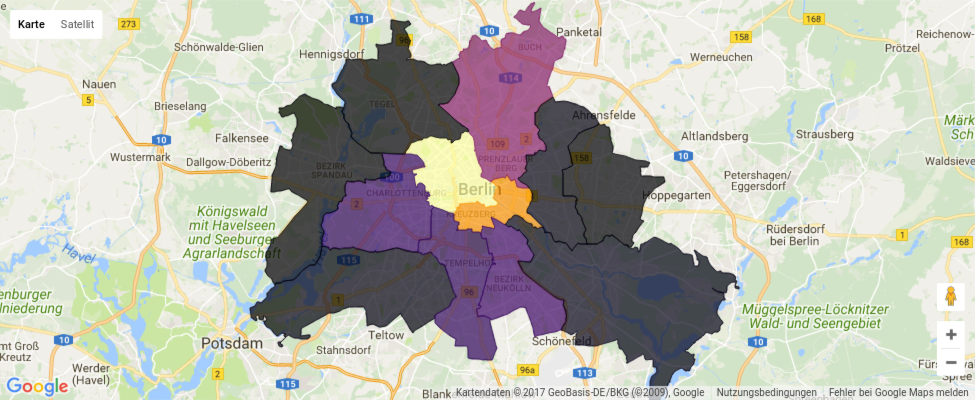
\includegraphics[width=0.49\linewidth]{images/activities_of_districts/Berlin.png}}\hfill
	\subfloat[Activity per Capita per District]{\label{fig1:b}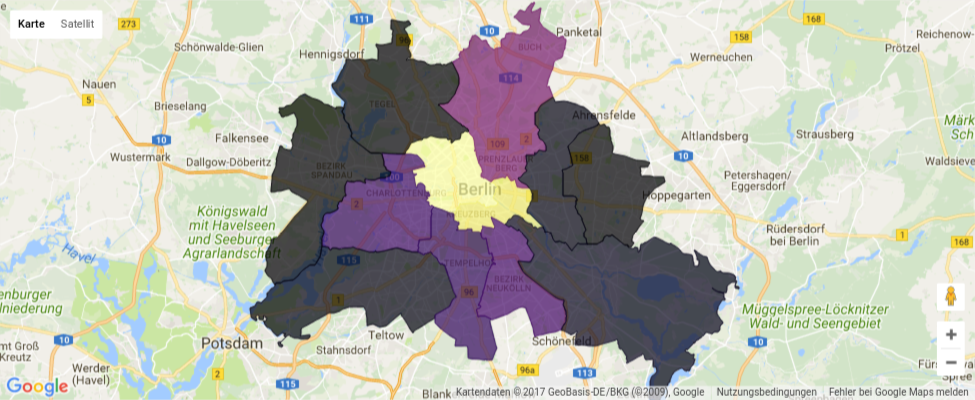
\includegraphics[width=0.49\linewidth]{images/activities_per_capita_of_districts/Berlin.png}}%
	\caption{Berlin}
\end{figure}


\begin{figure}[!htp]
	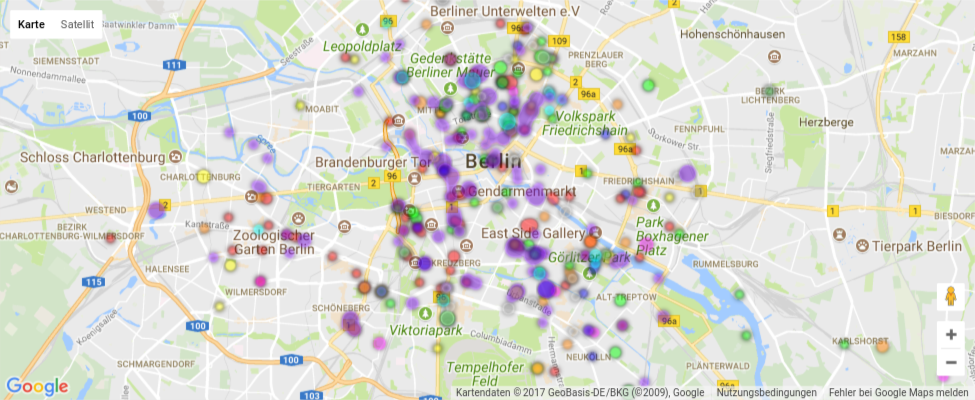
\includegraphics[width=1\linewidth]{images/Berlin_points.png}
	\caption{Snippet of Berlin with Open Events}\label{fig:berlinpoints}	
\end{figure}

Regarding the categories (\ref{fig:berlinbar}) it is obvious that the \emph{Tech} activities dominate in Berlin. The reason for this increased interest in technology may be due to a high number of upcoming startups. 
But actually the high dominance (three times larger than the second favorite; largest dominance) of technology events in contrast to other categories is a trait which all three examined German cities share. One conclusion would that Meetup seems so far to be limited to \emph{tech-interested} people in Germany. 

\begin{figure}[!htp]
	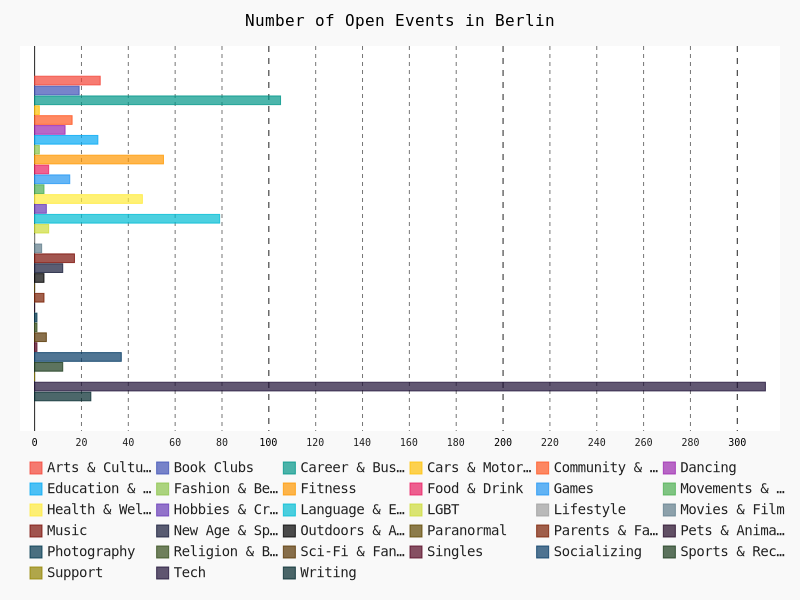
\includegraphics[width=1\linewidth]{../plotting/pngs/categories/Berlin.png}
	\caption{Activities per Category in Berlin}\label{fig:berlinbar}	
\end{figure}


\subsection*{Madrid}

Almost all events are concentrated in Madrid-Centro. Madrid's most favorite categories are by far Tech and Languages \& Ethnic Identity. 

\begin{figure}[!htp]
	% Maximum length
	\subfloat[Activity per District]{\label{fig1:a}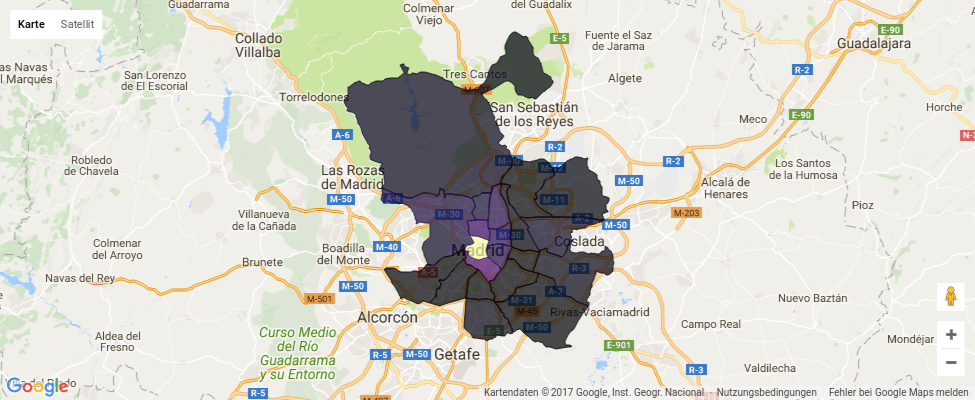
\includegraphics[width=0.49\linewidth]{images/activities_of_districts/Madrid.png}}\hfill
	\subfloat[Activity per Capita per District]{\label{fig1:b}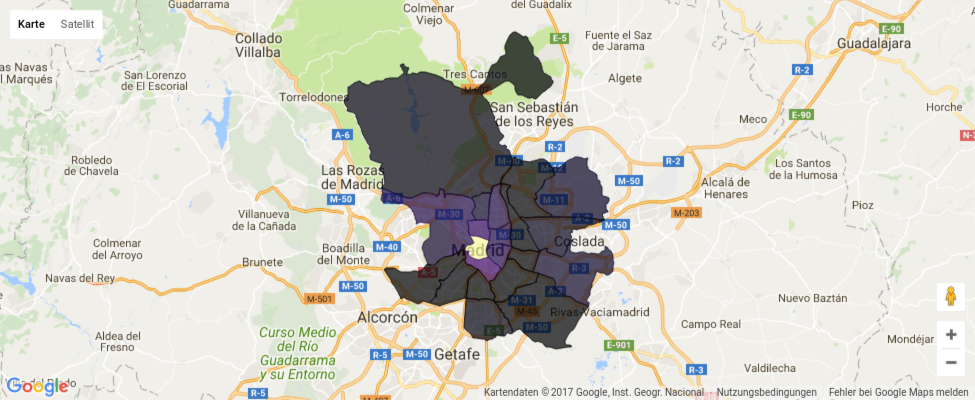
\includegraphics[width=0.49\linewidth]{images/activities_per_capita_of_districts/Madrid.png}}%
	\caption{Madrid}
\end{figure}

\subsection*{Paris}

Paris is an example for a more evenly distributed city - at least in the total number of events per district. This may be due to its small size and dense population (compare Barcelona). The picture would probably be different if one considers the vast metropolitan area of Paris with its 12 Mio. people and its area of 17000 $ km^2 $ (in contrast to the actual 2.2 Mio. and 105 $ km^2 $)
Again Tech and Language and Ethnic Identity are the most favored categories. 

\begin{figure}[!htp]
	% Maximum length
	\subfloat[Activity per District]{\label{fig1:a}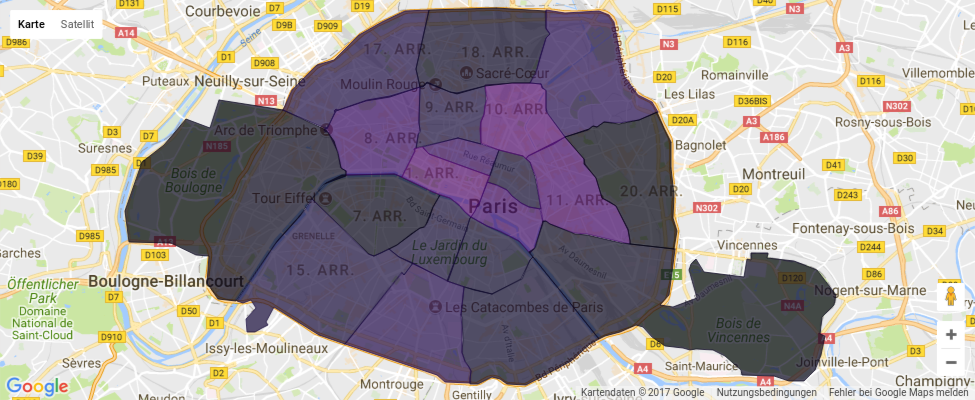
\includegraphics[width=0.49\linewidth]{images/activities_of_districts/Paris.png}}\hfill
	\subfloat[Activity per Capita per District]{\label{fig1:b}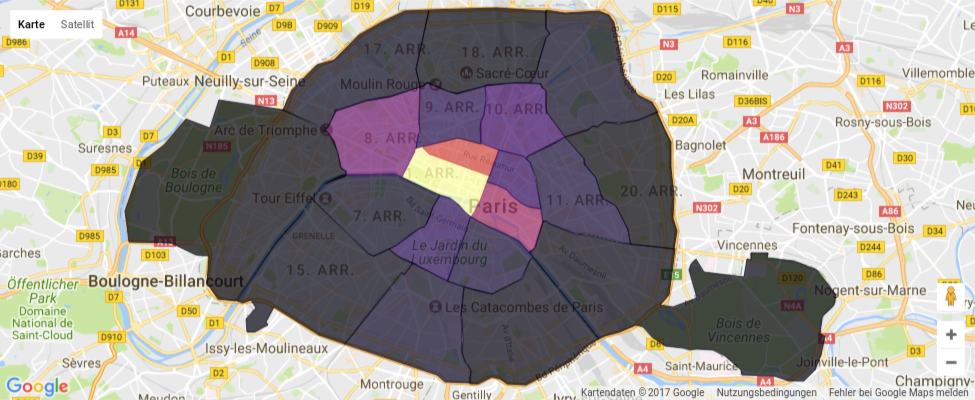
\includegraphics[width=0.49\linewidth]{images/activities_per_capita_of_districts/Paris.png}}%
	\caption{Paris}
\end{figure}


\subsection*{Brussels}

In this case we actually did not consider the City of Brussels but rather the Brussels-Capital Region. But one can clearly see the bright yellow shape which represents the City of Brussels (this is one \emph{district}!). Per capita some central regions like Ixelles show a higher activity too. 
\begin{figure}[!htp]
	% Maximum length
	\subfloat[Activity per District]{\label{fig1:a}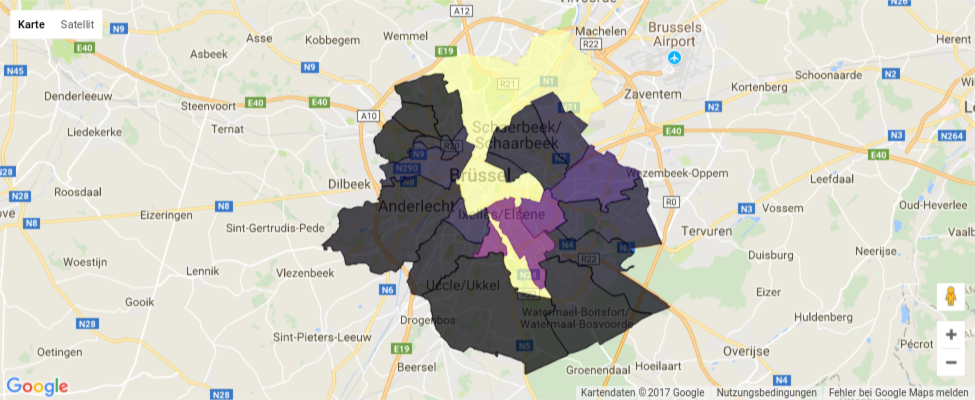
\includegraphics[width=0.49\linewidth]{images/activities_of_districts/Brussels.png}}\hfill
	\subfloat[Activity per Capita per District]{\label{fig1:b}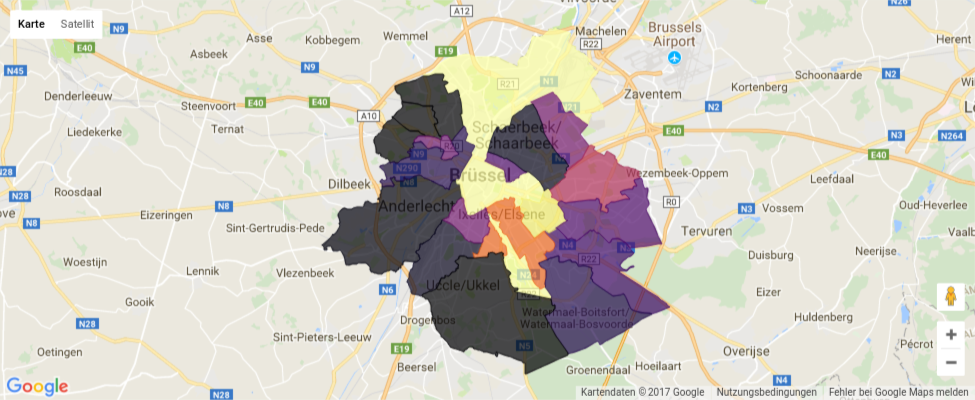
\includegraphics[width=0.49\linewidth]{images/activities_per_capita_of_districts/Brussels.png}}%
	\caption{Brussels}\label{fig:madridmap}
\end{figure}

\subsection*{Hamburg}
Hamburg is the second biggest city in Germany. As in Berlin mostly tech-interested people are using \url{Meetup.com}. Looking at the figures one can clearly identify the trending districts in Hamburg which are "Hamburg-Mitte" (middle), "Altona", "Eimsbüttel" and "Hamburg-Nord" (from west to east). One reason for this might be that lots of young people are living in these districts. For example, in "Hamburg-Mitte" there is the very famous "St. Pauli". In this part of the district a great part of the nightlife take place. Other districts like "Altona" and "Eimsbüttel" are trending as well since the University of Hamburg is located in "Rotherbaum" which is a part of "Eimsbüttel and close to "Altona", "Hamburg-Mitte" and "Hamburg-Nord".

\begin{figure}[!htp]
	% Maximum length
	\subfloat[Activity per District]{\label{fig1:a}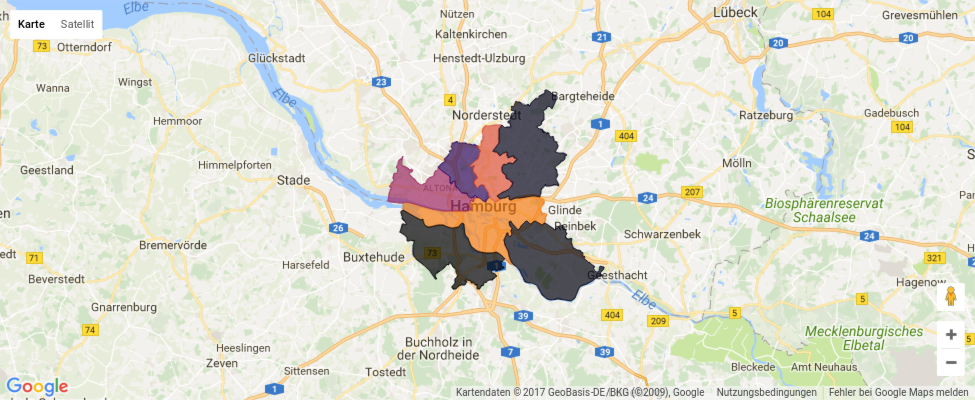
\includegraphics[width=0.49\linewidth]{images/activities_of_districts/Hamburg.png}}\hfill
	\subfloat[Activity per Capita per District]{\label{fig1:b}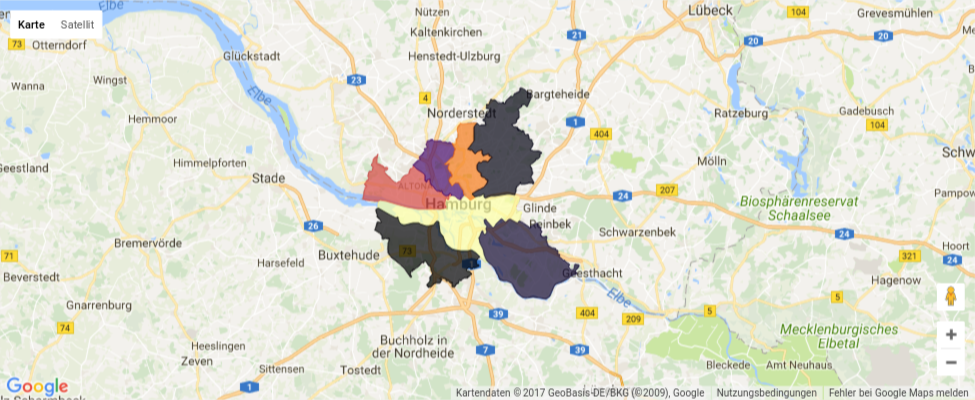
\includegraphics[width=0.49\linewidth]{images/activities_per_capita_of_districts/Hamburg.png}}%
	\caption{Hamburg}
\end{figure}

\subsection*{New York City}

The biggest city of the United States of America has the second largest amount of open events in our dataset. Here it is necessary to keep in mind that the real number of events can vary if the Meetup communities are more organized in closed groups. 

The picture New York shows is as one would expect. At least in the case for Manhattan which is by far \emph{the} center of the City with over 1000 open events. It is followed by the distant second Brooklyn less than one third of activities. Staten Island and the Bronx are hardly active. 

\begin{figure}[!htp]
	% Maximum length
	\subfloat[Activity per District]{\label{fig1:a}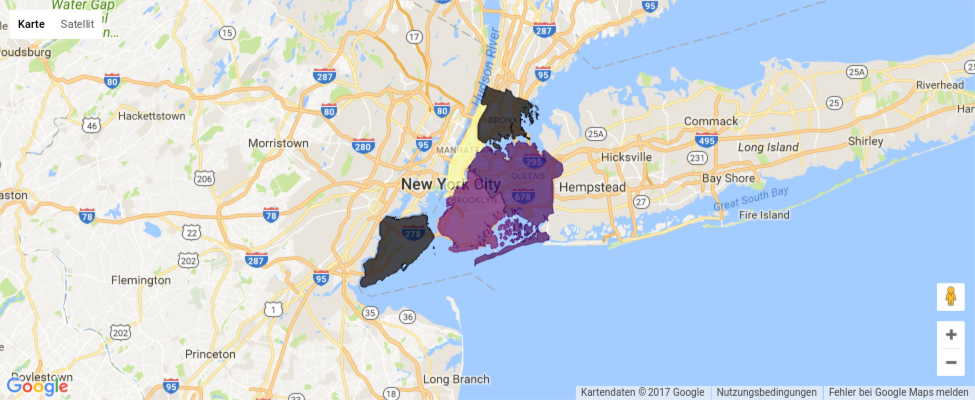
\includegraphics[width=0.49\linewidth]{images/activities_of_districts/NewYork.png}}\hfill
	\subfloat[Activity per Capita per District]{\label{fig1:b}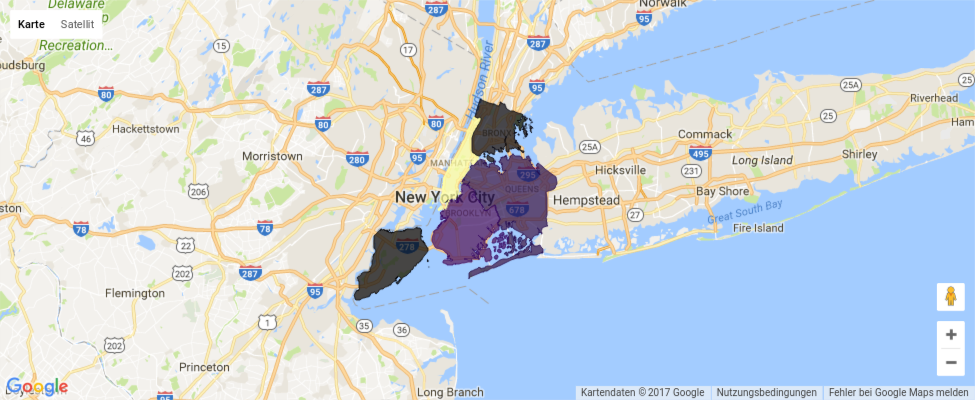
\includegraphics[width=0.49\linewidth]{images/activities_per_capita_of_districts/NewYork.png}}%
	\caption{New York City}\label{fig:newyorkmap}
\end{figure}

As \emph{Meetup Inc.} is based in New York it shows a diverse picture in regards to categories. The leading categories are Sports and Recreation, Tech, Career and Business and Socializing. 

\subsection*{Munich}

As the third German city in our set Munich does not seem to be much different than Berlin and Hamburg. Again most Meetup members are interested in Technology. In total number of activities Munich beats the more populated Hamburg and even Berlin if one considers activities per inhabitant. 

\begin{figure}[!htp]
	% Maximum length
	\subfloat[Activity per District]{\label{fig1:a}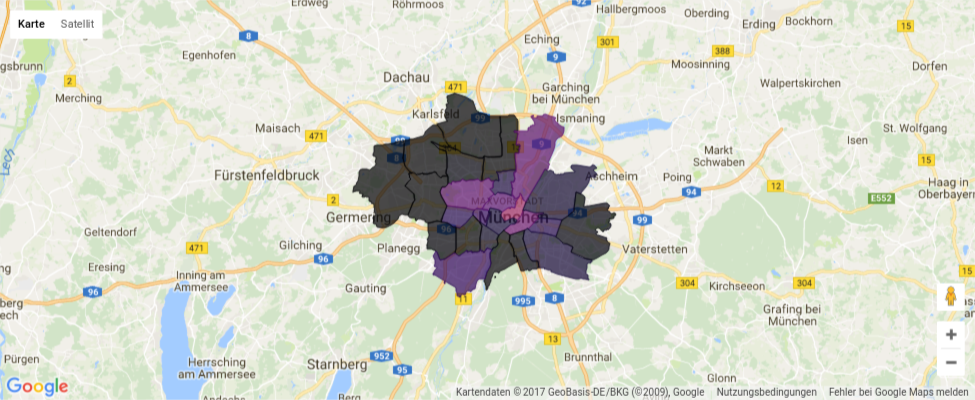
\includegraphics[width=0.49\linewidth]{images/activities_of_districts/Munich.png}}\hfill
	\subfloat[Activity per Capita per District]{\label{fig1:b}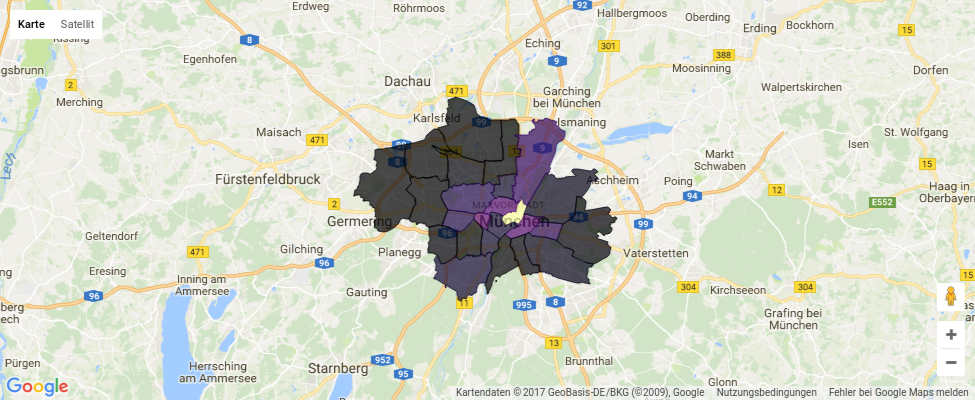
\includegraphics[width=0.49\linewidth]{images/activities_per_capita_of_districts/Munich.png}}%
	\caption{Munich}
\end{figure}

\subsection*{Hong Kong}

The first thing we notice is that Hong Kong has the lowest number of activities per capita in our dataset (compare Figure \ref{fig:categories_all_percapita}). It seems that \url{Meetup.com} did not reach Hong Kong and maybe the whole Chinese or even Asian market. 
As a business center it shows the largest activity in Socializing and Career and Business followed by Sports and Recreation. 

\begin{figure}[!htp]
	% Maximum length
	\subfloat[Activity per District]{\label{fig1:a}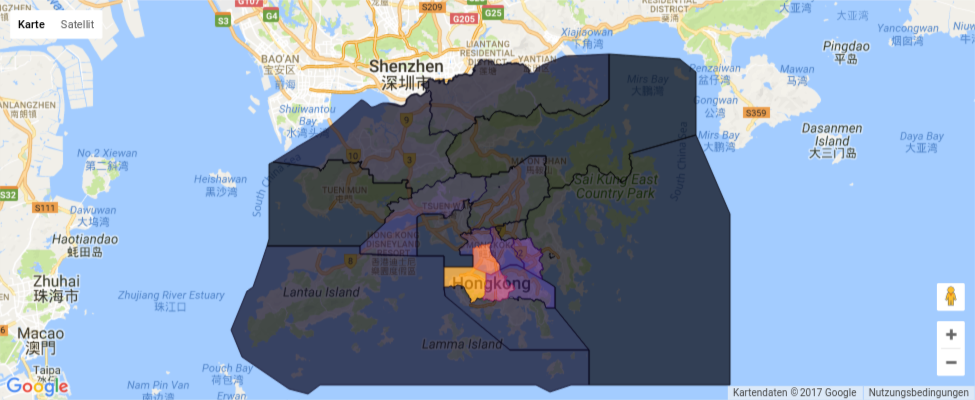
\includegraphics[width=0.49\linewidth]{images/activities_of_districts/HongKong.png}}\hfill
	\subfloat[Activity per Capita per District]{\label{fig1:b}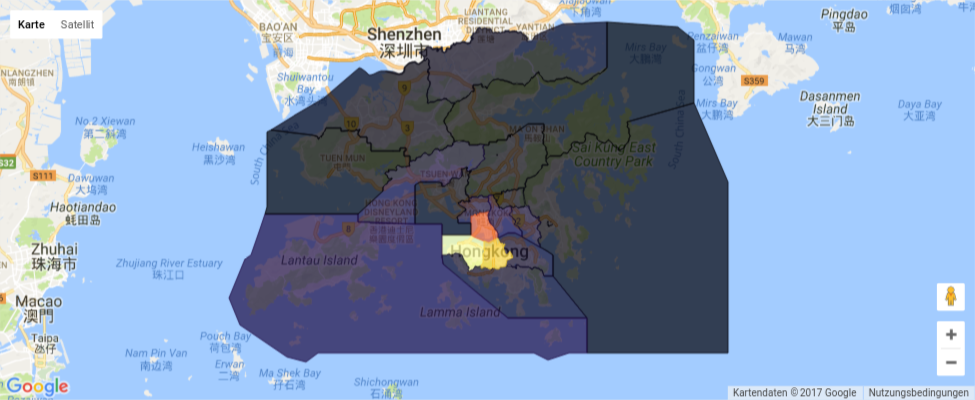
\includegraphics[width=0.49\linewidth]{images/activities_per_capita_of_districts/HongKong.png}}%
	\caption{Hong Kong}\label{fig:hongkongmap}
\end{figure}


\begin{figure}[!htp]
	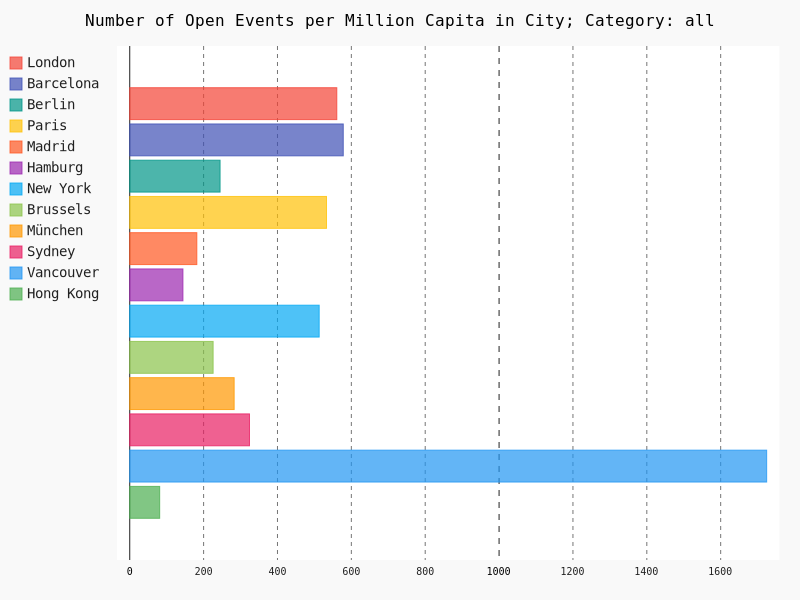
\includegraphics[width=1\linewidth]{../plotting/pngs/activities_per_city_per_capita/all.png}
	\caption{Number of Open Events in all Categories per Capita}\label{fig:categories_all_percapita}	
\end{figure}
